\begin{minipage}[b]{0.7\textwidth}

\begin{Exercise}[label  = rotierendes 3-Körper-Problem, difficulty = 4, label = cmrot, origin = {XX. IPhO 1989}, title = Starrer Körper]
	Drei (nicht-kolineare) Massen $m_i$ ($i \in \{1,2,3\}$) an Punkten $P_i$ wechselwirken ausschließlich gravitativ. Die durch diese drei Punkte aufgespannte Ebene sei $\nu$, und die dazu senkrecht stehende Rotationsachse $\sigma$. Welche Bedingungen müssen die drei Seitenlängen des Dreiecks $\Delta P_1P_2P_3$ ($a_{1,2}$; $a_{1,3}$; $a_{2,3}$) erfüllen, sodass dieses sich nicht verändert, also wie ein starrer Körper um $\sigma$ rotiert?
\end{Exercise}
\end{minipage}
\begin{minipage}[b]{0.3\textwidth}
	\centering
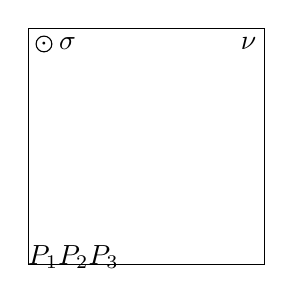
\begin{tikzpicture}
	\draw (0,0) rectangle (3,3);
	\node at (2.8,2.8) {$\nu$};
	\draw (0.2,2.8) circle (0.1);
	\node at (0.2,2.8) {$\cdot$};
	\node at (0.5,2.8) {$\sigma$};
	
	\tkzDefPoint(0.5,0.5){A}
	\tkzDefPoint(2.7,0.3){B}
	\tkzDefPoint(1.2,2.5){C}
	
	\tkzDrawPoints(A,B,C)
	\tkzLabelPoint[above](A){$P_1$}
	\tkzLabelPoint[above](B){$P_2$}
	\tkzLabelPoint[right](C){$P_3$}
	
	
\end{tikzpicture}
\end{minipage}
\begin{Answer}[ref = cmrot]
	Wir können uns zuerst überlegen, welche Bedingung die Winkelgeschwindigkeit $\omega$ erfüllen muss. Da sich die Körperabstände nicht ändern sollen, ist die potentielle Energie des Systems konstant. Da aber auch die Gesamtenergie erhalten bleibt, heißt das, dass auch die gesamte kinetische Energie konstant bleiben muss. Da sich aber bei einem starren Körper auch das Trägheitsmoment nicht ändern kann, heißt dass, das das System mit einer konstanten Winkelgeschwindigkeit $\omega$ rotieren muss.\\
	Wir geben nun die Positionen der drei Körper durch ihre Ortsvektoren $\mathbf{r_i}$ an. Dann wählen wir ein Koordinatensystem so, dass $\nu$ mit der $x-y-$Ebene zusammenfällt, und das $\sigma$ die $z-$Achse ist.\\
	In diesem Koordinatensystem ist der Schwerpunkt im Koordinatenursprung, es gilt also
	\begin{equation}\label{cmrot:com}
		\sum_{i=1}^{3} m_i\mathbf{r}_i = \mathbf{0}.
	\end{equation}
	Wir können jetzt o.B.d.A. die Kräfte betrachten, die auf den ersten Körper wirken. Das sind zum einen die Gravitationskräfte durch die Wechselwirkung mit Körper $2$ bzw. $3$ ($\mathbf{F}_{2}$ bzw. $\mathbf{F}_{3}$), als auch die im Inertialsystem wirkende Zentripetalkraft $\mathbf{F}_{z}$. Die Gravitationskräfte lassen sich durch die Seitenlängen im Dreieck ausdrücken:
	\begin{equation}\label{cmrot:grav}
		\mathbf{F}_2 = \frac{Gm_1m_2}{a_{1,2}^3}\left(\mathbf{r}_2-\mathbf{r}_1\right)~\mathrm{und}~\mathbf{F}_3 = \frac{Gm_1m_2}{a_{1,3}^3}\left(\mathbf{r}_3-\mathbf{r}_1\right).
	\end{equation}
	Die Zentripetalkraft ist gegeben durch
	\begin{equation}\label{cmrot:rot}
		\mathbf{F}_z = -m_1 \omega^2 \mathbf{r}_1,
	\end{equation}
	wobei $\omega$ die Winkelgeschwindigkeit ist.\\
	Im Kräftegleichgewicht, also bei konstater Rotation, muss nun gelten
	\begin{equation}\label{cmrot:fbal}
		\mathbf{F}_2 + \mathbf{F}_3 = \mathbf{F}_{z} \Rightarrow G \frac{m_1}{a_{1,2}^3} m_2 \mathbf{r}_2 + G \frac{m_1}{a_{1,3}}m_3\mathbf{r}_{3} + m_1 \mathbf{r}_1 \left(\omega^2 - \frac{Gm_2}{a_{1,2}^3} - \frac{Gm_3}{a_{1,3}}\right) = \mathbf{0}
	\end{equation}
	Gleichzeitig können wir \eqref{cmrot:com} umstellen nach
	\begin{equation}\label{cmrot:r2}
		m_2\mathbf{r}_2 = -m_1 \mathbf{r}_1 - m_3 \mathbf{r}_3.
	\end{equation}
	Wenn wir das jetzt wieder in \eqref{cmrot:fbal} einsetzen, kommen wir auf
	\begin{equation}\label{cmrot:ncl}
		\mathbf{r}_1m_1 \left(\omega^2 - \frac{Gm_2}{a_{1,2}^3} - \frac{Gm_3}{a_{1,3}^3} - \frac{Gm_1}{a_{1,2}^3}\right) + \mathbf{r}_{3} \left(\frac{1}{a_{1,3}^3} - \frac{1}{a_{1,2}^3} \right) = \mathbf{0}.
	\end{equation}
	Da nach Voraussetzung die Vektoren $\mathbf{r}_1$ aber nicht kolinear seien soll, ist die einzige Möglichkeit, dass eine Linearkombination von ihnen wie in \eqref{cmrot:ncl} den Nullvektor ergibt, dass die Koeffizienten null sind.\\
	Aus dem zweiten Term kommen wir jetzt auf 
	\begin{equation}\label{cmrot:el}
		\frac{1}{a_{1,3}^3} - \frac{1}{a_{1,2}^3} \overset{!}{=} 0 \Rightarrow a_{1,2} = a_{1,3}:= a.
	\end{equation}
	Der erste Term führt zu
	\begin{equation}
		\omega^2 a^3 = GM,
	\end{equation}
	mit $M = m_1+m_2+m_3$. \\
	Wenn wir den gleichen Spaß jetzt für die anderen beiden Körper machen, kommen wir darauf, dass alle drei Seiten gleich lang sein müssen, und die Bewegung nur dann als starrer Körper stattfinden kann, wenn alle drei mit konstanter Winkelgeschwindigkeit in Form eines gleichseitigen Dreiecks rotieren.
\end{Answer}
